% This is samplepaper.tex, a sample chapter demonstrating the
% LLNCS macro package for Springer Computer Science proceedings;
% Version 2.20 of 2017/10/04
%
\documentclass[runningheads]{llncs}
%
\usepackage{graphicx}
\usepackage{hyperref}
\renewcommand\UrlFont{\color{blue}\rmfamily}
\setlength{\parskip}{0pt}
\raggedbottom
\usepackage{multirow}
\usepackage{amsmath}
\usepackage{csquotes}
\usepackage{paralist}
\usepackage{booktabs}
\usepackage{mathptmx}
\usepackage{pgfplots}
\pgfplotsset{compat=1.8}
\usepackage{subfigure}
\pgfplotsset{width=7cm,compat=1.8}
\usepackage{pgfplotstable}
\renewcommand*{\familydefault}{\sfdefault}
\usepackage{tikz}

\begin{document}
\title{Prediction of Malaria with Machine Learning Algorithms : An experimental Study}

%%
%% The "author" command and its associated commands are used to define
%% the authors and their affiliations.
%% Of note is the shared affiliation of the first two authors, and the
%% "authornote" and "authornotemark" commands
%% used to denote shared contribution to the research.
\author{Ousseynou Mbaye \and Mouhamadou Lamine Ba  \and Alassane Sy}
%
\authorrunning{Ousseynou Mbaye \and M. Lamine Ba  \and Alassane Sy}
% First names are abbreviated in the running head.
% If there are more than two authors, 'et al.' is used.
%
\institute{Universit\'e Alioune Diop de Bambey, Bambey, Senegal\\
\email{firstmidlle.last@uadb.edu.sn}
}



%%
%% By default, the full list of authors will be used in the page
%% headers. Often, this list is too long, and will overlap
%% other information printed in the page headers. This command allows
%% the author to define a more concise list
%% of authors' names for this purpose.
%\renewcommand{\shortauthors}{O. Mbaye et al.}

%%
%% The abstract is a short summary of the work to be presented in the
%% article.

%%
%% The code below is generated by the tool at %%http://dl.acm.org/ccs.cfm.
%% Please copy and paste the code instead of the example below.
%%


%%
%% Keywords. The author(s) should pick words that accurately describe
%% the work being presented. Separate the keywords with commas.



%
\maketitle              % typeset the header of the contribution
%
\begin{abstract}

Still today, Malaria remains one of the most feared diseases in Sub- Saharan Africa and especially in Senegal. This is mainly due to inappropriate medical care support coupled with an often late and error-prone diagnosis from the medical staff. In addition, largely used diagnostic standards such as the Rapid Diagnosis Test is not fully reliable. With the development and increasing adoption of automated tools in the health field, machine learning applications might help medical actors in their decision-making process. In this paper, we propose an experimental study of six machine learning algorithms for the prediction of Malaria in Senegal. These algorithms aim at predicting whether or not a given patient suffers from Malaria based on his signs and symptoms. The performance of the algorithms have been extensively tested and evaluated over real data sets about patients in Senegal that suffer or not from Malaria. The algorithms are evaluated using four criteria: accuracy, Recall, F-measure, Precision and Specificity. The research has shown that there is not necessarily a single best classification tool, but instead the best performing algorithm will depend on the dataset to be analysed
 
\end{abstract}
%
%
% Introduction
\section{Introduction}\label{intro}
Malaria is one amongst the most deadly disease in the world, especially in sub-saharan Africa countries such as Senegal.
Malaria is caused by parasitic single-celled microorganisms belonging to the Plasmodium group; it is an infectious
disease which is transmitted to human being through bites from infected female Anopheles mosquitoes. Someone who suffers
from  Malaria may present symptoms that typically include fever, tiredness, vomiting, and headaches. In its severe form,
the disease can cause yellow skin, seizures, coma or death.

\subsubsection{Studied problem and motivations.}
According to the last report \cite{Wh17}  about the propagation of Malaria disease around the world, published in November 2017 by the World international Health Organization (WHO in short),
 216 millions of cases have been reported in 2016. As a result, the number of cases has significantly increased when compared to the 211 millions of reported Malaria patients in 2016.
As for the number of death due to Malaria, it does not decrease between 2016 and 2017 (446.000 vs. 445.000) despite the huge effort made by governements
and non-governmental organization to improve healthcare services and the awareness strategies, especially in critical areas. 
When analyzing the statistics above in details, one can easily notice that the burden of the Africa region of the World 
international Health Organization is colossal. Indeed, 90\% of Malaria cases and 90\% of deaths due to the disease were located in this area in 2016.
More specifically, 80\% of the burden in terms of morbidity is distributed in fifteen countries, all located in Sub-saharan Africa except India. This demonstrates
that Malaria is a real flail in Sub-saharan Africa states and Senegal is not spared at all. We investigate in this study an efficient approach to predict, using machine learning, the occurence 
or not of Malaria when a patient has to be diagnosed. Given the patient signs and symptoms, as well as the result from the quick diagnosis test, our solution should be to 
automatically tell if she suffers from Malaria or not with a high accuracy.

Malaria is an acute problem in Senegal  due mainly to the lack of high quality healthcare services and well-formed
staffs able to perform accurate diagnosis of diseases that patients suffer from. Over the past years, the government with 
the help of international organizations have tried to eradicate Malaria by implementing various proactive and reactive solutions 
to fill the gap in terms of services and human resources. However, the mortality rate is still very high, e.g. in underserved areas,
areas without required healthcare needs, uneducated people, population with low income, etc. Most of these deaths cases are reported to be caused by inaccurate diagnosis, sometimes 
incomplete leading to a bad prediction of the exact type of Malaria.
On the other hand, Malaria occurence or complication can often occur during  popular events (for instance religious events such as the Grand Magal of Touba \cite{So17})
which gather thousands of persons from everywhere in the country during a short time period. During those popular events, non-permanent medical points are set in order
to assist and treat ill persons; the staff in a given health point might be formed sometimes by only volunteers without advanced medical skills. Each of these medical 
points might receive and treat hundreds of patients each day with some of them potentially suffering from Malaria. 
This appeals for the need of finding automated tools to help medical actors in their decision making process, and thereby to improve provided 
healthcare services.   

\subsubsection{Proposed diagnosis approach.}
In this paper we present first steps towards an efficient manner to automatically diagnosis Malaria occurence or not based on patient signs and symptoms,
and the outcome from the quick diagnosis test. We define our diagnosis task as a classical binary classification problem by considering two classes: \textquote{Malaria} and \textquote{not-Malaria}.
Given a patient data, our main goal is to properly find to which class the patient belongs. To solve this classification problem we rely on machine learning and use the logistic regression
function as the basis of our prediction approach. Machine learning has been largely used in several domains (e.g. Health Informatics  \cite{Du13}) for various purposes whereas logistic regression has demonstrated its efficiency when dealing with a binary classification problem. 
 
As an application scenario, we focus on predicting Malaria cases in Senegal. At this end, we use  a large volume of patient record dataset collected during the most popular religious event in Senegal from the different installed health points, namely more than twenty points that deadly receive hundreds of patients.
As an immediate result of this work, we introduce a data preparation pipeline in order to 
\begin{inparaenum}[(i)]
\item explore the dataset for profiling purpose;
\item only retain records related to Malaria;
\item clean and transform attributes, as well data values, into the extracted Malaria dataset; and 
\item impute missing values (there were lot of missing values in the collected health dataset as reported in Section\ref{data_prep}).
\end{inparaenum}
Such a data preparation pipeline has been realized using \emph{OpenRefine} (formely Google Refine) to perform various cleaning and profiling tasks on our raw atient dataset and \emph{missForest}, a robust
 algorithm for imputing  missing data of diverses types; see Section \ref{data_prep} for more details. 
Expermients on the real world patient dataset, augmenting with a semi-synthetic dataset, show promising performance results regarding the effectiveness of the proposed approach.

\subsubsection{Paper organization.}The remaining of the paper is organized as follows. We summarize the related work on data imputation and binary classification methods in Section \ref{related_work}.
In Section \ref{data_prep} we introduce a data preparation pipeline on the raw collected patient records for the prediction phase. 
We then present our prediction model for Malaria cases in Section \ref{prediction_model}.
Experiments and performance analysis  on the collected real-world dataset, as well as a semi-synthetic dataset,  are detailled in Section \ref{experimentation} before we conclude in Section \ref{conclusion}. 


% Prediction Model
\section{Review of evaluated ML algorithms}\label{ml_algorithms}

We mainly provide a brief overview of Machine Learning and Deep Learning models for healthcare applications. \\

In healthcare, Machine Learning apps can help better understand each patient's care journey, medical decisions, or the impact of new drugs. Today researchers are using machine learning algorithms in the diagnosis of several diseases such as diabetes, stroke, cancer, malaria and heart disease. In the following we discuss about some of these methods.  Those algorithms are chosen among the most used ones in the health field according to studies\cite{de2018binary,tomar2013survey}.\\
 %Decision tree
\textbf{Decision tree (DT)}\cite{Ro05} is a supervised classifier which is obtained by recursively partitioning the labelled set of observations. It is one of the most adopted classifiers, thanks to its simplicity and its straightforward interpretation. For CART algorithms, hyperparameters are the impurity criteria (entropy and gini), the maximum depth, the minimum samples to split and the minimum samples at a leaf
Decision tree algorithm has been applied in many medical tasks, for examples, in increasing quality of dermatologic diagnosis[11], predicting essential hypertension [12], and predicting cardiovascular disease [13], predict and diagnose of heart disease [14].Decision tree is one of the most popular tools for classification and prediction.\\
% Random forest
\textbf{Random Forest (RF)}\cite{Be01} is an ensemble approach built upon many decision tree classifiers. It is a supervised classifier which requires the same hyper parameters as DT, plus the number of trees to create and the random number of features to look at when splitting the labelled data during the training step \cite{Be01}.\\
% Naive Bayes
\textbf{ Naive Bayes classifier (NB) }\cite{Ka17} is a\emph{supervised} machine learning algorithm, i.e. requires to be trained, used for classifying observations to given distinct classes based on \emph{input explanatory variables} (a.k.a feature or attribute).
It is a classification technique based on the well-known \emph{Bayes’ theorem}\footnote{https://en.wikipedia.org/wiki/Bayes\%27\_theorem} with strong and naive assumptions. It simplifies learning by assuming that features are independent of given class.
The Bayesian classifier has been applied in many medical issues, for examples, in measuring quality of care in psychiatric emergencies [21], predicting and diagnosis heart disease [14]. and assisting diagnosis of breast cancer [22].\\
% Logistic Regression 
\textbf{Logistic regression (LR)} \cite{Ph88} is a statistical model used in the machine learning domain as a supervised classifier for binary classification \cite{uddin2019comparing}. 
It is based, in its basic form, on a logistic function to describe a binary dependent variable\cite{wang2014support,de2018binary} by considering as input 
qualitative or/and ordinal explanatory variables  in order to measure the probability of a given class label. The greatest advantage  of the logistic regression
classifier is the fact that you can use continuous explanatory variables and it is easier to handle more than two explanatory variables simultaneously and its ability to quantify the strength of the relationship between each explicative variable and the variable to explain, given the other variables integrated to the model. One the other hand, the logistic regression is one of the most used multi-valued models in epidemiology[23]. In such a context, the variable to explain is often the occurrence or not of an event like a disease and the explanatory variables, i.e. the features, are those that highly impact the occurrence of this event, i.e. variables assessing the exposure to a risk factor or a protective factor, or a variable representing the confusion factor. The logistic regression is applied to predict malaria in [26] and in identification of at-risk populations in public health research and outreach [27] and the results are  are very relevant.\\
%Support Vector Machine
\textbf{Support Vector Machine (SVM)} \cite{Ev01} is a supervised classification approach whose intuition is to represent input data in a space and to determine the optimal hyper-plane that divides that space in two regions depending on the targeted value.
SVM is used to studied the diagnosis of coronary artery disease[28].\\
% artificial neural networks
\textbf{An Artificial Neural Network (ANN)} \cite{Me19} is a computational approach also referred to as a Connectionist System used in Machine Learning. ANNs are loosely modeled after the biological neural network in an attempt to replicate the way in which we learn as humans. Think of it as a computing system, structured as a series of layers, each layer consisting of one or several neurons. The types of the layers comprise \emph{input}, \emph{output} and \emph{hidden} layers \cite{anderson1972simple,raschka2015python}.

% Related work
\section{Related work}\label{related_work}
In this section, we summarize the sate-of-the-art research on Malaria in general, and in particular the
use of machine learning techniques to tackle the various aspects related to one of the 
major healthcare problems worldwide which is Malaria.

% Studies on Malaria
As it is well-known, Malaria is caused by the bite of the female Anopheles, the most dangerous of which
is Plasmodium falciparum. Many early works have been consequently focused on the study of the evolution and
the distribution of the responsible mosquito, mainly with the goal to detect or diagnosis the severity of the 
disease given an infected patient \cite{Fe03,Al09}. Recent research on Malaria have largely adopted machine learning
and showed its ability to solve various aspects of the disease. Most of these machine learning based techniques are 
based on the analysis of blood data obtained from high-definition microscopic screenshots as in \cite{Ku18}. The authors
in \cite{Ku18} propose an unsupervised learning algorithm that detects and determines the types of infected blood cells.
Used prediction approach consists of quantifying the amount of plasmodium parasites in a blood smear. In the same research intuition
of harnessing blood, the Jordan-Elman neural network classifier introduced in \cite{Ha15}, on the other hand, to quickly determine the occurrence 
of Malaria and its severity level as well: the neural network analyzes the features of the blood data of the patients.  
Still using ML, DIAZ et al. have proposed in \cite{Dia09} a semi-supervised algorithm enable to quantify and classify the 
erythrocytes infected by Malaria parasistes through microscopic images. The orginiality of this work comes from its usability
even in the presence of thin blood drandruff infected by falciparum Plasmodium for the quantification and the classificationi tasks.
Besides blood data, sign and symptom records were also used to study Malaria with ML methods. Indeed, decision trees based approach
has been proposed in Nigeria \cite{Ug10} to predict the occurrence of Malaria given diagnostic data. However a decision tree suffers 
from various limitations as a classifier. Indeed it can easily overfit or can be extremely sensitive to small pertubations in data for instance.
Even though we both rely on signs and symptoms, the prediction model in \cite{Ug10} differs from ours on numerous facets: our model is built upon
logistic regression and is trained using also inputs from the quick diagnosis test. In addition, we apply our method in the context of patients living in Senegal. 
An example of previous work that has used logistic regression is that of Farida et al. in \cite{Ad10}. The logistic regression is exploited
there for the selection of features in order to construct stable decision trees. The decision trees are then used to predict the severity
criteria of Malaria in the context of Afghanistan. 


In the same line of works applying machine learning, in \cite{Pr17}, Pranav et al. propose Malaria likelihood prediction model built on a deep reinforcement learning (RL) agent. 
Such a RL predicts the probability of a patient testing positive for Malaria using answers from questions about their household. In 
the presented approach the authors have also dealt with the problem of determining the right question to ask next as well as the length of the survey, dynamically.
Moreover, statistically enhanced rule-based classification model to diagnose malaria has been proposed in \cite{Bb16}. A corresponding prototype 
which incorporates the rules and statistical models have been implemented; the main goal of the study was to develop a statistical 
prototype to perform clinical diagnosis of malaria given its adverse effects on the overall healthcare, yet its treatment remains 
very expensive for the majority of the patients to afford.

To the best of our knowledge this is the first work in Senegal that attempts to provide a prediction model for identifying 
the occurrence of Malaria given patient data.  


% Data Preparation
\input{datasets}



% Experimentation and Results
\section{Experimentation and results}\label{experimentations}
We detail and analyze in the section the results of the experimentation we performed using the six ML algorithms presented in Section \ref{ml_algorithms} over the two real datasets described in Section \ref{datasets}. We start by presenting our experimentation setting.

% experimentation setting
\subsection{Experimentation Setting}
In this section data is available for applying classification algorithm. After model creation from training data, classification operation is performed on test data. 
All the performed tests have been done in the same machine and the same operating system. To test the performance of our six chosen ML algorithms, we relied on their Python implementations available through the scikit-learn library. Scikit-learn is an open source simple and efficient tool for predictive data analysis that implements most of the existing ML algorithms

Then some of the most important performance evaluation measures like accuracy, precision, sensitivity, specificity, F-measure and area under ROC curve are evaluated and compared. 
For the details about the description of each parameter of ML we refer to the official documentation of the implementation of these algorithms in scikit-learn7. Concerning the segmentation of both datasets for the training of our ML algorithms and their testing we have considered the stratified-5-fold cross-validation in classification model construction and efficiency evaluation. This method is very useful to handle data with an unbalanced class distribution, increases the validation of classification and prevents from random and invalid results.


% Results of the experiments
\subsection{Results of the experiments}

This section presents the results of the experimentation on each real dataset for each of the six classifiers. 
\subsubsection{Decision Tree}

Table 1  below shows the performance measures (precision, recall, F measure and precision) of the results of our Decision Tree classifier after experimentation on all our datasets. The observation shows that the best scores of our classifier are achieved on the datasets DT1, DT3 and DT5 which are 97.04\%, 80.86\% and 83.41\% respectively. Also AUC (Area Under the Curve) values are higher for these same datasets which are 0.78, 0.86 and 0.76 respectively. However, we note that the sensitivity values are higher than the specificity values on the datasets DT1, DT3  and DT5 whereas they are substantially lower than thoses of datasets DT2 and DT4. This means that DT is more inclined to predict as well whether a given patient has malaria or he doesn’t, on the datasets DT2, DT3 and DT4, while our classifier on the datasets DT1 and DT5 our classifier is only efficient in predicting whether a given patient has malaria. This same trend is observed on the F-scores which higher values varying between 0.91 and 0.98 on the datasets DT1, DT3 and DT5.

% Decision Tree
\begin{table}[!ht]
\centering
\begin{tabular}{*{7}{c}l r}
  \toprule
  \textbf{Datasets} & \textbf{Precision} & \textbf{Recall} & \textbf{F1-score}&\textbf{AUC} &\textbf{Score}&\textbf{Specificity}\\
   \midrule
  DT1 &0.97  & 1   & 0.98 & 0.78 & 97.04 & 0.05 \\
  DT2 & 0.59 &0.48 &0.48  &0.64  &63.01  &0.80\\
  DT3 &0.89  &0.85 &0.87  &0.86  &80.86  &0.69\\
  DT4 &0.68  &0.57 &0.62  &0.70  &65.60  &0.74\\
  DT5 &0.99  &0.84 &0.91  &0.76  &83.41  &0.58\\

  
    \bottomrule
\end{tabular}
\caption{Performances measures of DT over all datasets}\label{perf-measure-dt1}
\end{table}
\subsubsection{Random Forest}
The performance of the random forest varied throughout the study depending on the dataset, although overall it performed well as shown in Table 2. Notice that best accuracy are achieved by random forest classifier on the datasets DT1, DT2 and DT5 which are respectively 97.13\%, 80.86\% and 78.35\%. In contrast with the results obtained with the DT classifier, the Sensivity values are higher than specificity values on datasets DT1 and DT5 whereas the inverse is noticed on the dataset DT3. At the same time we note that these values are roughly identical on the datasets DT3 and D4
%Random Forest
\begin{table}[!ht]
\centering
\begin{tabular}{*{7}{c}l r}
  \toprule
  \textbf{Datasets} & \textbf{Precision} & \textbf{Recall} & \textbf{F1-score}&\textbf{AUC} &\textbf{Score} &\textbf{Specificity}\\
   \midrule
  DT1 &0.97 &1   &0.99 &0.81 &97.13& 0.07\\
  DT2 &0.63  & 0.34  &0.44&0.64&63.33& 0.85\\
  DT3 &0.89 &0.85 &0.87&087&80.86&0.70\\
  DT4 &0.68 &0.56&0.62&0.70&65.82&0.74\\
  DT5 &0.99 &0.84&0.91&0.76&78.35&0.60\\
  
  
    \bottomrule
\end{tabular}
\caption{Performances measures of RF over all datasets}\label{perf-measure-dt1}
\end{table}


%Logistic Regression
\subsubsection{Logistic Regression}

Logistic regression In table 3 we show the performance measures LR classifier experimented on our five datasets. We notice that our classifier have overall precision which are vary between 58\% and 98\%. 

\begin{table}[!ht]
\centering
\begin{tabular}{*{7}{c}l r}
  \toprule
  \textbf{Datasets} & \textbf{Precision} & \textbf{Recall} & \textbf{F1-score}&\textbf{AUC} &\textbf{Score}&\textbf{Specificity}\\
   \midrule
  DT1 &0.97 &1   &0.99 &0.79 &97.19&0.05 \\
  DT2 & 0.58 &0.36   &0.44&0.63&61.96&0.81\\
  DT3 &0.85 &0.88 &0.86&0.86&79.59&0.55\\
  DT4 &0.98 &0.56&0.92&0.70&65.82&0.72\\
  DT5 & 0.90&0.78&0.88&0.84&81.86&0.75\\
  
  
    \bottomrule
\end{tabular}
\caption{Performances measures of LR over all datasets}\label{perf-measure-dt1}
\end{table}
We observe that the higher precision is obtained with DT4 dataset while the corresponding score is equal to 65.82\% is the lowest of all other datasets. Also we notice that the LR presents homogeneous results on the DT3 dataset with an accuracy of 85\%, a sensitivity equal to 88\%, an F-score of 92\%, an AUC which is 0.86 and a score equal to 79.59\%. . We also note that the best AUC and the best F-score are obtained by LR on the DT3 dataset.
\subsubsection{Naives Bayes}
In contrast with the results above, NB classifier presents very heterogeneous performances regarding the performance measures used as shown in Table 4. In fact, we observe that the best precision is achieved on the dataset DT5 which is 99\%, although the best F-score and the higher accuracy are obtained on the dataset DT1 which are 0.99 and 97.13\% respectively and finally the best AUC is observed on the dataset DT3 which is 0.85. We also note that the best specificity is obtained on DT4 and varies between 0.65 and 0.70 (see appendices).
\begin{table}[!ht]
\centering
\begin{tabular}{*{7}{c}l r}
  \toprule
  \textbf{Datasets} & \textbf{Precision} & \textbf{Recall} & \textbf{F1-score}&\textbf{AUC} &\textbf{Score}&\textbf{Specificity}\\
   \midrule
  DT1 &0.97 &1   &0.99 &0.81 &97.13 &0.00\\
  DT2 & 0.60 &0.34   &0.43&0.63&62.86&0.83 \\
  DT3 &0.86 &0.87 &0.86&0.85&79.94&0.60\\
  DT4 &0.68 &0.59&0.63&0.70&65.63&0.73\\
  DT5 &0.99 &0.82&0.90&0.84&85.61&0.71\\
  
  
    \bottomrule
\end{tabular}
\caption{Performances measures of NB over all datasets}\label{perf-measure-dt1}
\end{table}
\subsubsection{Support Vector Machine}
%SVM

Table 5 shows the performance measures of the SVM classifier.
\begin{table}[!ht]
\centering
\begin{tabular}{*{7}{c}l r}
  \toprule
  \textbf{Datasets} & \textbf{Precision} & \textbf{Recall} & \textbf{F1-score}&\textbf{AUC} &\textbf{Score}&\textbf{Specificity}\\
   \midrule
  DT1 &0.97 &1   &0.99 &0.84 &97.13&0.00 \\
  DT2 &0.58  &0.05   & 0.09&0.62&62.86&0.97\\
  DT3 &0.57 & 0.86&0.86&0.85&79.94&0.64\\
  DT4 & 0.68&0.58&0.62&0.70&65.63&0.73\\
  DT5 &0.99 &0.86&0.92&0.80&85.61&0.62\\
    \bottomrule
\end{tabular}
\caption{Performances measures of SVM over all datasets}\label{perf-measure-dt1}
\end{table}
Table 1 shows the performance measures. The observation shows that the best score, precision and F1-score are obtained on the datasets DT1, DT3 and DT5. However the higher AUC and the best specificity are observer on the datasets DT1, DT3 and DT4.
%ANN
\subsubsection{Artificial Neural Nework}
The performance of the ANN varied throughout the study depending on the dataset, although overall it performed well. A large amount of initial effort was required to train and validate the model. Notice that best precision are achieved by ANN classifier on the datasets DT1, DT3 and DT5 which are respectively 97\%, 89\% and 99\%. While the higher AUC and the best scores are obtained on the datasets DT1 and DT3. The Sensivity values are higher than specificity values on datasets 
\begin{table}[!ht]
\centering
\begin{tabular}{*{8}{c}l r}
  \toprule
  \textbf{Datasets} & \textbf{Precision} & \textbf{Recall} & \textbf{F1-score}&\textbf{AUC} &\textbf{Score}&\textbf{Specificity}\\
   \midrule
  DT1 &0.97&1 &0.99   &0.84 &97.15&0.04  \\
  DT2 &0.59  &0.40   &0.48&0.65&62.86&0.80 \\
  DT3 &0.89 &0.85 &0.87&0.87&86.68&0.69\\
  DT4 &0.68 &0.58&0.62&0.70&0.70&0.75\\
  DT5 &0.99 &0.84&0.91&0.79&83.26&0.65\\ 
    \bottomrule
\end{tabular}
\caption{Performances measures of ANN over all datasets}\label{perf-measure-dt1}
\end{table}

\subsection{Discussion}
In this study, the algorithms DT, RF, LR, NB, SVM and ANN were applied on five datasets concerning patients with or without malaria and living in regions of Senegal namely: Diourbel, Thies and Fatick. Indeed, in order to offer a new technique for diagnosing and predicting malaria, it is important to know the performance of those existing through our datasets.
Analysing in details the performance of our six classifiers across the five datasets, the results show that there is not necessarily a single best classification algorithm, but that the best performing algorithm will depend on the characteristics of the dataset to analyze. Indeed we notice that all the algorithms produce their best precision on the DT1, DT3, and DT5 data sets. These values, which reach 97\% at times, outperform the Rapid Diagnosis Test which is the standard diagnostic tool largely adopted in the healthcare system in Senegal.
\begin{figure}
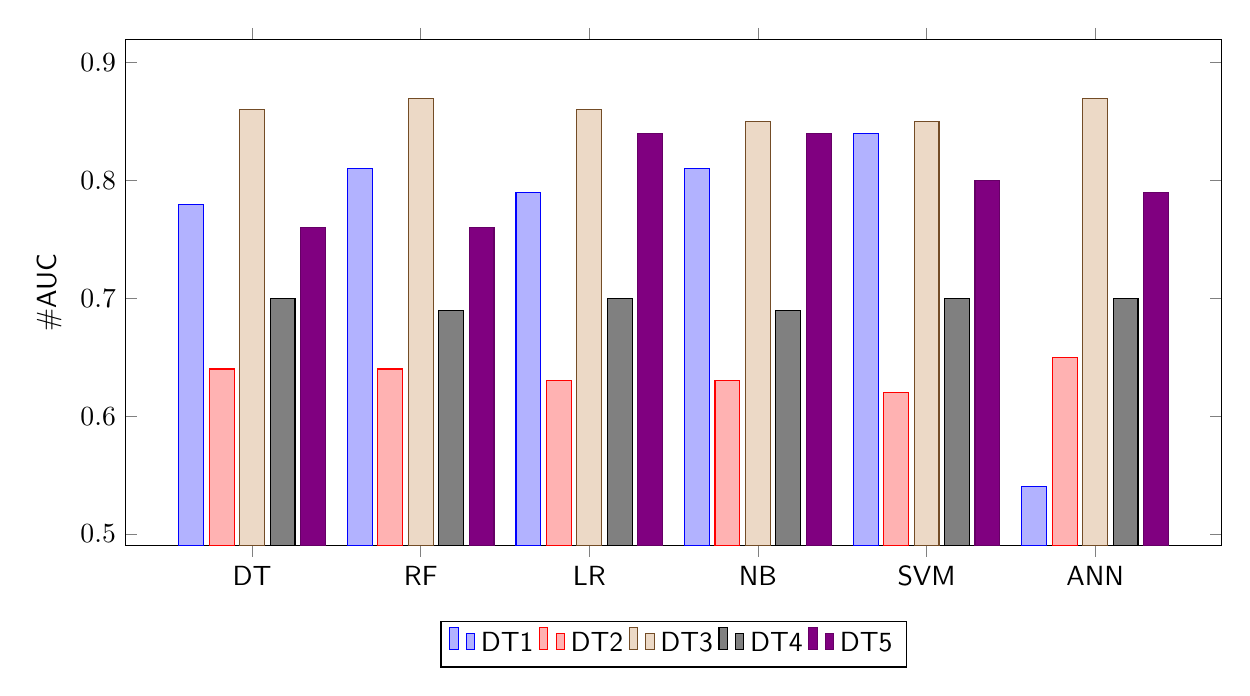
\begin{tikzpicture}
 \centering
\begin{axis}[
    height=8cm, width=15.5cm,
    bar width=0.4cm,
    ybar,
    %ybar=5pt,% configures `bar shift'
    bar width=9pt,
    enlargelimits=0.15,
    legend style={at={(0.5,-0.15)},
    anchor=north,legend columns=-1},
    ylabel={\#AUC},
    symbolic x coords={{DT,RF,LR,NB,SVM,ANN}},
    xtick=data,
    %nodes near coords,
    nodes near coords align={vertical},
    ]
\addplot coordinates {(DT,0.78) (RF, 0.81) (LR,0.79)(NB, 0.81)(SVM,0.84)(ANN, 0.54)};
\addplot coordinates{(DT,0.64) (RF, 0.64) (LR,0.63)(NB, 0.63)(SVM,0.62)(ANN, 0.65)};
\addplot coordinates {(DT,0.86) (RF, 0.87) (LR,0.86)(NB, 0.85)(SVM,0.85)(ANN, 0.87)};
\addplot coordinates {(DT,0.70) (RF, 0.69) (LR,0.70)(NB, 0.69)(SVM,0.70)(ANN, 0.70)};
\addplot coordinates {(DT,0.76) (RF, 0.76) (LR,0.84)(NB, 0.84)(SVM,0.80)(ANN, 0.79)};
\legend{DT1,DT2,DT3,DT4,DT5}
\end{axis}
\end{tikzpicture}
\caption{comparison of Roc Area achieved by six classifiers}
\end{figure}
However, on these same datasets, the algorithms often present very low specificities, for example 0.05 on DT1. This shows that our best performing classifiers are only able to predict a single class: either the patient has malaria or he does not, but not in both spots. This is because the DT1 and DT3 datasets are very unbalanced. In fact in these datasets either the number of patients with malaria is greater than those who are not or the opposite is true. Furthermore, we note that on the DT2 and DT4 datasets all the algorithms present specificities and Sensivity that are significant and quite similar. Contrary to what is quoted a little above, on these datasets the algorithms are efficient on the prediction tasks of the two classes. Looking closely at the results in terms of precision, recall and F-measure we observe that the classifiers RF, LR, SVM and ANN generally outperform the others for each dataset. Indeed, for the dataset DT1, which contains observations on patients living in different regions of Senegal, these four classifiers have an accuracy of 99\%, a recall greater than 92\% and an F-measure greater than 95\%. We note the same trend with the DT2 dataset which contains observations on patients living in the same area in Senegal. It can also be noted that RF, LR, SVM and ANN have better precision than the rapid diagnostic test carried out and systematically used in the majority of health structures in Senegal. This observation remains true with DT4 which is a perfectly balanced dataset. In conclusion, it is very difficult or even impossible for us to say definitively which algorithm is more efficient for the task of predicting malaria, but the choice of this one will strongly depend on the choice of the data set. However, this study shows that our classification problem has been taken care of. A method integrating several models and various datasets is necessary

\begin{figure}
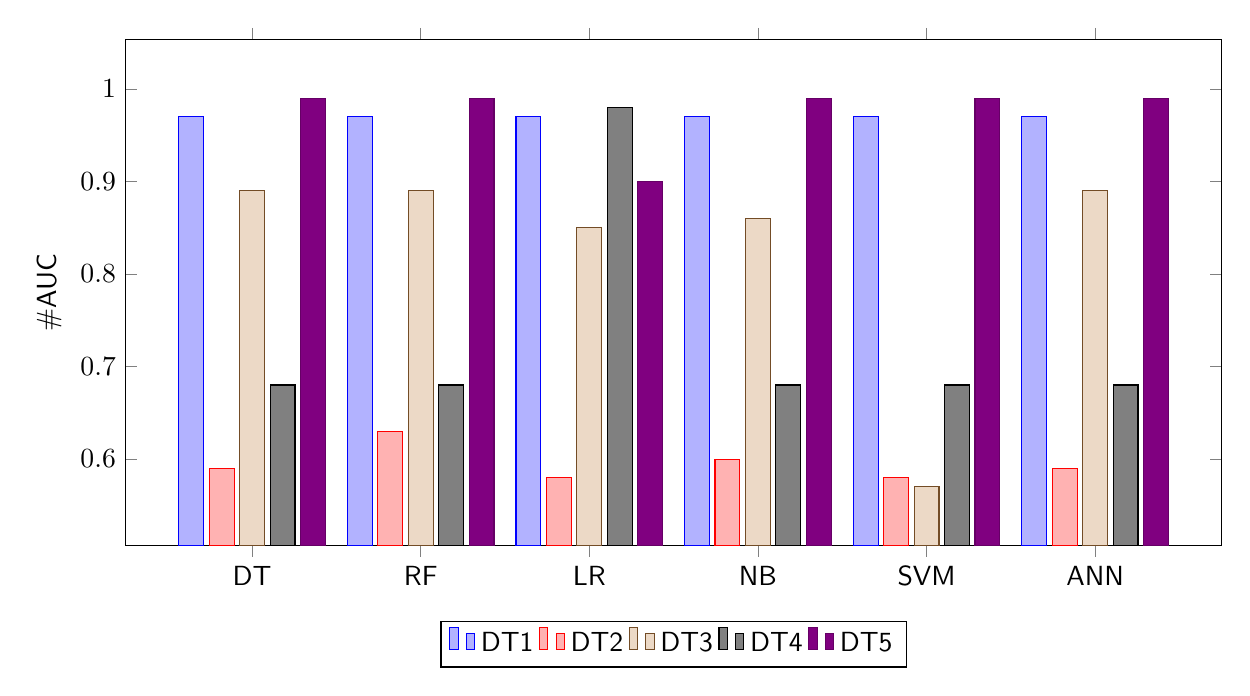
\begin{tikzpicture}
 \centering
\begin{axis}[
    height=8cm, width=15.5cm,
    bar width=0.4cm,
    ybar,
    %ybar=5pt,% configures `bar shift'
    bar width=9pt,
    enlargelimits=0.15,
    legend style={at={(0.5,-0.15)},
    anchor=north,legend columns=-1},
    ylabel={\#AUC},
    symbolic x coords={{DT,RF,LR,NB,SVM,ANN}},
    xtick=data,
    %nodes near coords,
    nodes near coords align={vertical},
    ]
\addplot coordinates {(DT,0.97) (RF, 0.97) (LR,0.97)(NB, 0.97)(SVM,0.97)(ANN, 0.97)};
\addplot coordinates{(DT,0.59) (RF, 0.63) (LR,0.58)(NB, 0.60)(SVM,0.58)(ANN, 0.59)};
\addplot coordinates {(DT,0.89) (RF, 0.89) (LR,0.85)(NB, 0.86)(SVM,0.57)(ANN, 0.89)};
\addplot coordinates {(DT,0.68) (RF, 0.68) (LR,0.98)(NB, 0.68)(SVM,0.68)(ANN, 0.68)};
\addplot coordinates {(DT,0.99) (RF, 0.99) (LR,0.90)(NB, 0.99)(SVM,0.99)(ANN, 0.99)};
\legend{DT1,DT2,DT3,DT4,DT5}
\end{axis}
\end{tikzpicture}
\caption{comparison of Precision achieved by six classifiers}

\end{figure}


\begin{figure}
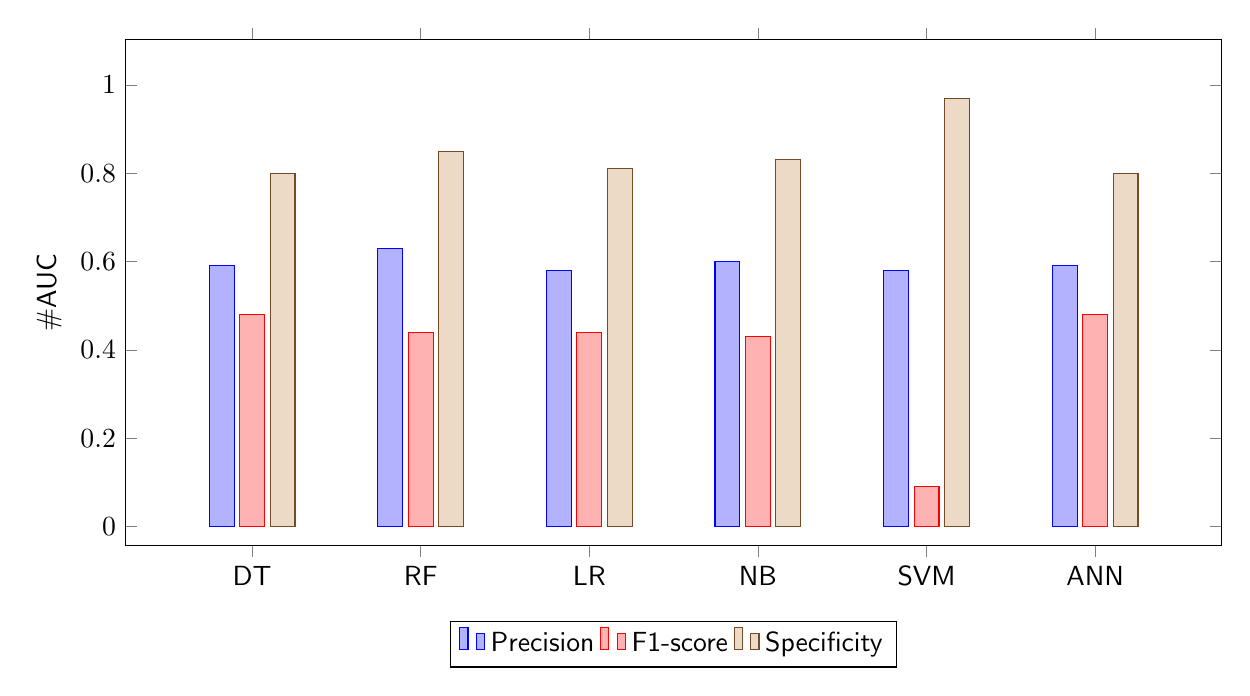
\begin{tikzpicture}
 \centering
\begin{axis}[
    height=8cm, width=15.5cm,
    bar width=0.4cm,
    ybar,
    %ybar=5pt,% configures `bar shift'
    bar width=9pt,
    enlargelimits=0.15,
    legend style={at={(0.5,-0.15)},
    anchor=north,legend columns=-1},
    ylabel={\#AUC},
    symbolic x coords={{DT,RF,LR,NB,SVM,ANN}},
    xtick=data,
    %nodes near coords,
    nodes near coords align={vertical},
    ]
\addplot coordinates {(DT,0.59) (RF, 0.63) (LR,0.58)(NB, 0.60)(SVM,0.58)(ANN, 0.59)};
\addplot coordinates{(DT,0.48) (RF, 0.44) (LR,0.44)(NB, 0.43)(SVM,0.09)(ANN, 0.48)};
\addplot coordinates {(DT,0.80) (RF, 0.85) (LR,0.81)(NB, 0.83)(SVM,0.97)(ANN, 0.80)};
%\addplot coordinates {(DT,0.68) (RF, 0.68) (LR,0.98)(NB, 0.68)(SVM,0.68)(ANN, 0.68)};
%\addplot coordinates {(DT,0.99) (RF, 0.99) (LR,0.90)(NB, 0.99)(SVM,0.99)(ANN, 0.99)};
\legend{Precision,F1-score,Specificity,DT4}
\end{axis}
\end{tikzpicture}
\caption{comparison of other performance measures in classifiers on DT1}

\end{figure}

% Conclusion
\section{Conclusion}\label{conclusion}
In this study, six ML models have been extensively tested and compared over various datasets in order to evaluate their performance for the task of predicting Malaria occurrence in a patient knowing his signs and symptoms. The results obtained show that some of them are promising and overcome RDT in particular settings. As future work, we plan to study the implementation of an ensemble method for predicting Malaria occurrence built on the algorithms offering the best performances in our present study. 

%
% ---- Bibliography ----
%
% BibTeX users should specify bibliography style 'splncs04'.
% References will then be sorted and formatted in the correct style.
%
\bibliographystyle{splncs04}
\bibliography{biblio}
%

\end{document}
